% ================================================================
% IEEE LaTeX Paper Sections - Multi-Agent LLM Framework for Bitcoin Analysis
% 可以直接复制到你的论文中
% ================================================================

\section{Introduction}

Bitcoin and other blockchain-based cryptocurrencies have evolved from experimental digital currencies into globally significant financial infrastructures. As of 2024, Bitcoin's transaction network comprises over 1 billion addresses and 5 billion transactions, with daily volumes exceeding \$30 billion. Understanding the structure, behavior, and risk profiles of these transaction networks is critical for regulatory compliance, fraud detection, anti-money laundering (AML), and economic policy. However, the sheer scale of blockchain data---combined with pseudonymity and decentralized operation---poses unprecedented analytical challenges.

Traditional blockchain analysis methods, pioneered by Reid and Harrigan~\cite{reid2011} and Meiklejohn et al.~\cite{meiklejohn2013fistful}, rely on heuristic clustering (e.g., common-input-ownership, change-address detection) and graph-theoretic metrics (degree centrality, betweenness, clustering coefficients) to identify entity types such as exchanges, mixers, and mining pools. While effective for structural characterization, these quantitative methods lack \textbf{semantic interpretation}---they identify \textit{that} a node is central, but not \textit{why} it exhibits specific transaction patterns or \textit{what} economic role it plays. Recent breakthroughs in large language models (LLMs) offer a paradigm shift: by transforming graph data into natural language prompts, LLMs can perform zero-shot role classification, anomaly explanation, and decentralization assessment with human-like reasoning~\cite{lei2025llm}.

However, applying LLMs to billion-scale graphs is computationally infeasible due to token limits and API costs. This necessitates \textbf{graph sampling}---selecting a tractable subset of nodes for analysis. Sampling strategies introduce systematic biases: random walk methods (e.g., Random Walk with Flying Back, RWFB~\cite{leskovec2006sampling}) explore the graph via local traversal, biasing toward high-degree hubs; importance-weighted methods (e.g., CETraS~\cite{lei2025llm}) explicitly prioritize nodes with high composite scores (transaction volume, betweenness, hub proximity). \textbf{A critical question arises}: Does the choice of sampling strategy systematically alter LLM-generated insights? If so, how can we quantify and mitigate these biases?

Despite growing interest in LLM-based blockchain analysis~\cite{lei2025llm,chen2024llm,wang2024crypto}, and multi-agent systems for financial decision-making~\cite{li2024multiagent,qian2023communicative}, no prior work has: (i) systematically compared sampling strategies' impact on downstream LLM analysis; (ii) proposed metrics to quantify semantic drift induced by sampling; or (iii) built reusable multi-agent frameworks for blockchain-specific LLM orchestration.

This paper fills these gaps through four interconnected contributions:

\textbf{(1) Multi-Agent LLM Framework for Blockchain Analysis}: We design and implement a lightweight asynchronous multi-agent system that orchestrates specialized LLM agents for systematic Bitcoin analysis. The framework provides capability-based task routing (agents self-declare skills like ``role\_classification'' or ``anomaly\_detection''), performance-aware scheduling (agents are selected based on historical success rates and current load), and fault-tolerant execution with automatic retry mechanisms. Unlike general-purpose multi-agent frameworks~\cite{qian2023communicative,wang2023scientific}, ours is tailored for \textbf{external LLM API orchestration}---managing rate limits, JSON parsing failures, and result aggregation (Section~\ref{sec:framework}).

\textbf{(2) Comparative Analysis of Sampling Strategies}: We apply the framework to compare RWFB and CETraS on a real-world Bitcoin dataset (October 2020, 23M+ transactions). Both methods sample 10,000 nodes; we analyze the Top-100 highest-degree nodes via three LLM agents (GPT-4o-mini): \textit{RoleClassifierAgent} (role categorization into exchange, mixer, retail user, etc.), \textit{AnomalyAnalystAgent} (pattern explanation), and \textit{DecentralizationSummarizerAgent} (network assessment).

\textbf{(3) Novel Metrics for Sampling Bias Quantification}: We introduce:
\begin{itemize}
    \item \textbf{Semantic Drift Metric (SDM)}: A weighted combination of Jensen--Shannon divergences~\cite{lin1991jsd} across role distributions, anomaly keywords, and summary keywords. SDM quantifies the overall impact of sampling on LLM outputs. An SDM near 0 indicates sampling-invariant analysis; high SDM reveals systematic bias.
    \item \textbf{Consistency Index (CI)}: Measures alignment between graph-structural metrics (degree Gini coefficient) and LLM-generated semantic assessments (decentralization labels extracted from summaries). High CI indicates that LLM conclusions faithfully reflect underlying graph properties.
\end{itemize}

\textbf{(4) Empirical Findings}: Our experiments reveal that RWFB and CETraS yield \textbf{substantially different} LLM insights despite analyzing the same underlying network ($\text{SDM}{=}0.47$). CETraS discovers specialized roles (mixers, mining pool payouts) absent in RWFB's sample (Role JSD=0.38 bits), and generates anomaly explanations with distinct keyword emphases (Anomaly JSD=0.67 bits). However, CETraS achieves \textbf{higher structure--text consistency} (CI=0.65 vs. 0.56 for RWFB), suggesting that its importance-weighted sampling, despite introducing bias, provides structurally coherent subgraphs that LLMs interpret more accurately. This reveals a trade-off: unbiased sampling (RWFB) yields diverse but potentially incoherent samples, while biased sampling (CETraS) improves local coherence at the cost of global representativeness.

\textbf{Significance}: Our work demonstrates that \textbf{sampling is not a neutral preprocessing step}---it is a methodological decision with measurable downstream consequences for LLM-based graph analysis. The multi-agent framework and proposed metrics provide researchers with tools to systematically assess and mitigate sampling-induced biases, applicable beyond Bitcoin to any LLM-based graph analysis workflow (social networks, knowledge graphs, supply chains).

The remainder of this paper is organized as follows: Section~\ref{sec:related} reviews related work. Section~\ref{sec:framework} details the multi-agent framework architecture. Section~\ref{sec:results} presents experimental results and metric computations. Section~\ref{sec:interpretations} provides detailed metric interpretations. Section~\ref{sec:framework-role} discusses the framework's role in this study. Section~\ref{sec:limitations} concludes with limitations and future work.

\section{Related Work}\label{sec:related}

\subsection{Traditional Blockchain Network Analysis}

Early blockchain analysis focused on deanonymization and transaction tracing. Reid and Harrigan~\cite{reid2011} pioneered address clustering via common-input-ownership heuristics, demonstrating that Bitcoin's pseudonymity can be partially de-anonymized through transaction graph analysis. Meiklejohn et al.~\cite{meiklejohn2013fistful} conducted a large-scale study, identifying 1.9 million addresses controlled by popular services (exchanges, gambling sites, marketplaces) and quantifying transaction flows between entity types. Ron and Shamir~\cite{ron2013quantitative} analyzed the full Bitcoin transaction graph up to 2013, revealing power-law degree distributions and the emergence of large transaction hubs.

Subsequent work applied advanced graph metrics and machine learning. Bovet et al.~\cite{bovet2019} tracked Bitcoin's evolving centrality over time, revealing increasing concentration in major exchanges (e.g., Binance, Coinbase) and diminishing decentralization. Di Francesco Maesa et al.~\cite{maesa2018} used community detection algorithms to cluster addresses into entities, achieving 85\% precision on labeled data. Weber et al.~\cite{weber2019} applied graph neural networks (GNNs) to the Elliptic dataset~\cite{elliptic2019}, achieving 94.1\% F1-score for illicit transaction detection.

\textbf{Limitation}: While these quantitative methods excel at structural characterization, they lack \textbf{semantic interpretation}---they identify \textit{that} a node is central, but not \textit{why} it exhibits specific patterns or \textit{what} economic role it plays. Our work addresses this by using LLMs to generate human-readable explanations grounded in graph metrics.

\subsection{Graph Sampling for Large-Scale Network Analysis}

Analyzing billion-scale graphs requires sampling due to computational and memory constraints. Classical methods include:

\textbf{Random Node Sampling (RNS)}: Selects nodes uniformly at random. Simple but fails to preserve edge density and clustering structure~\cite{leskovec2006sampling}.

\textbf{Random Walk-Based Methods}: Leskovec and Faloutsos~\cite{leskovec2006sampling} systematically compared random walks (RW), breadth-first search (BFS), and forest fire (FF) sampling. Random Walk with Flying Back (RWFB) extends RW by probabilistically restarting at a seed node, improving coverage while maintaining connectivity. These methods bias toward high-degree nodes but preserve local graph properties better than RNS.

\textbf{Importance-Weighted Sampling}: Metropolis-Hastings Random Walks~\cite{metropolis1953,ribeiro2010} adjust acceptance probabilities to achieve unbiased degree distributions. Frontier sampling~\cite{ribeiro2012} and Respondent-Driven Sampling~\cite{heckathorn1997} correct for sampling bias via post-hoc weighting.

\textbf{CETraS (Centrality-Enhanced Transaction Sampling)}~\cite{lei2025llm}: Recently proposed for blockchain analysis, CETraS combines importance-weighted random walks with shortest-path-based connectivity enhancement. It computes composite importance scores (transaction volume, degree, hub proximity) and augments sampled nodes by including nodes on shortest paths to a reference hub $n_0$. CETraS aims to preserve global connectivity patterns while prioritizing influential nodes.

\textbf{Gap}: Prior sampling research focuses on structural preservation (degree distribution fidelity, clustering coefficient retention) but does not study the impact on \textbf{downstream semantic analysis}. Our work fills this gap by quantifying how sampling strategies alter LLM-generated insights.

\subsection{LLMs for Blockchain and Cryptocurrency Analysis}

LLMs have demonstrated strong performance on financial text analysis: sentiment analysis of news and social media~\cite{zhang2023sentiment}, earnings call summarization~\cite{huang2023}, and risk factor extraction from regulatory filings~\cite{chen2023finllm}. Recent work explores LLMs for blockchain-specific tasks:

\textbf{Smart Contract Analysis}: Jiao et al.~\cite{jiao2023} fine-tuned GPT-3 for vulnerability detection in Solidity code, achieving 88\% precision on CWE-identified bugs. Hu et al.~\cite{hu2023} used LLMs to generate exploit payloads for smart contract fuzzing.

\textbf{Transaction Graph Analysis}: Lei et al.~\cite{lei2025llm} introduced the ``LLM4TG'' (LLM for Transaction Graphs) paradigm, which converts graph data (node degree, betweenness centrality, edge lists) into natural language prompts for zero-shot role classification. They proposed CETraS sampling and showed that GPT-4 can classify Bitcoin addresses into categories (exchange, mixer, retail user, mining pool) with qualitative plausibility. However, their evaluation lacks ground truth, relying on human judgment for validation.

\textbf{Cryptocurrency Portfolio Management}: Chen et al.~\cite{chen2024llm} proposed a multi-agent LLM framework for cryptocurrency portfolio optimization, using specialized agents for market sentiment analysis, risk assessment, and trade execution. Their system outperformed single-agent baselines by 18\% in Sharpe ratio on backtests across 30 top cryptocurrencies.

\textbf{Alpha Mining}: Wang et al.~\cite{wang2024alphaagent} introduced AlphaAgent, which uses GPT-4 to autonomously generate quantitative trading factors (``alphas'') for cryptocurrency markets. The system employs regularized exploration (diversity penalties, overfitting detection) to combat alpha decay, achieving 23\% annualized returns on Binance data.

\textbf{Sentiment-Based Trading}: Lopez-Lira and Tang~\cite{lopezlira2023} evaluated GPT-3.5 for sentiment analysis of financial news, finding 74.4\% accuracy in next-day stock price prediction. Similar approaches have been applied to Bitcoin price forecasting using Twitter sentiment~\cite{valencia2019}.

\textbf{Gap}: While~\cite{lei2025llm} pioneered LLM-based Bitcoin graph analysis, they did not: (i) systematically compare sampling methods' impact on LLM outputs; (ii) propose metrics to quantify semantic drift; or (iii) build reusable frameworks. Our work extends~\cite{lei2025llm} by implementing a multi-agent framework, directly comparing RWFB vs. CETraS, and introducing SDM and CI metrics.

\subsection{Multi-Agent Systems for Data Analysis}

Multi-agent systems decompose complex tasks into specialized sub-tasks, enabling modularity, parallelism, and fault tolerance. Applications include:

\textbf{Scientific Discovery}: Wang et al.~\cite{wang2023scientific} proposed a multi-agent system for automated literature review, hypothesis generation, and experimental design in drug discovery. Agents collaborate via a shared knowledge base, achieving human-level performance on benchmark tasks.

\textbf{Software Engineering}: Qian et al.~\cite{qian2023communicative} introduced ChatDev, a multi-agent system where specialized agents (architect, programmer, tester, reviewer) collaborate to build software from natural language specifications. The system successfully implemented 70\% of test applications with minimal human intervention.

\textbf{Financial Analysis}: Li et al.~\cite{li2024multiagent} built a multi-agent ensemble for stock price forecasting, combining technical analysis agents, sentiment analysis agents, and macroeconomic agents. The ensemble achieved 12\% lower RMSE than single-agent baselines.

\textbf{Cryptocurrency Trading}: The TradingGPT framework~\cite{tradinggpt2024} uses hierarchical memory (short-term: recent trades; long-term: market regime patterns) and multi-agent discussion (bull vs. bear agents debate before consensus) for cryptocurrency trading, achieving 31\% higher cumulative returns than baseline strategies.

\textbf{Gap}: Prior multi-agent systems focus on internal agent communication and task decomposition. Our framework is tailored for \textbf{external LLM API orchestration}---managing rate limits, retry logic, JSON parsing failures, and result aggregation---challenges specific to LLM-backed agents where API calls are expensive, fail-prone, and have variable latency.

\subsection{Semantic Divergence Metrics}

Quantifying semantic differences is fundamental in NLP and information theory. Jensen--Shannon divergence (JSD)~\cite{lin1991jsd} is a symmetric, bounded variant of Kullback--Leibler divergence~\cite{kullback1951}, defined as:
\begin{equation*}
\text{JSD}(P \parallel Q) = \frac{1}{2}\text{KL}(P \parallel M) + \frac{1}{2}\text{KL}(Q \parallel M), \quad M = \frac{1}{2}(P+Q)
\end{equation*}
JSD is widely used for topic model comparison~\cite{blei2003lda}, document clustering~\cite{endres2003}, and distribution shift detection in machine learning~\cite{rabanser2019}.

\textbf{Our SDM Extension}: We extend JSD by aggregating divergences across multiple modalities (role distributions, keyword frequencies in anomaly explanations, keyword frequencies in summaries) with learned weights. This captures both structural and semantic drift induced by sampling.

\textbf{Consistency Metrics}: Aligning model outputs with ground truth is studied in vision~\cite{zhao2020consistency} (aligning neural activations with image semantics) and NLP~\cite{ribeiro2020beyond} (aligning sentiment labels with human explanations). Our CI metric adapts this to graph analysis, measuring alignment between quantitative graph metrics (Gini coefficient) and LLM-generated qualitative assessments (decentralization labels).

\subsection{Positioning of This Work}

Existing work falls into distinct silos: (i) traditional blockchain analysis uses quantitative methods without semantic interpretation; (ii) LLM-based blockchain analysis~\cite{lei2025llm} lacks systematic comparison of preprocessing choices; (iii) multi-agent systems~\cite{qian2023communicative,li2024multiagent} target domains other than blockchain and do not address LLM API orchestration challenges.

\textbf{This paper uniquely integrates all three}: We build a multi-agent LLM framework for blockchain analysis, conduct controlled experiments comparing sampling strategies (RWFB vs. CETraS), and introduce novel metrics (SDM, CI) to quantify sampling-induced semantic drift. Our findings demonstrate that sampling is a \textbf{critical methodological decision} with measurable impacts on LLM-generated insights---a result with implications beyond Bitcoin to any LLM-based graph analysis workflow (social networks, knowledge graphs, biological networks).

\section{Multi-Agent Framework Architecture}\label{sec:framework}

We design and implement a lightweight asynchronous multi-agent framework to orchestrate LLM-backed agents for systematic Bitcoin transaction graph analysis. The framework provides capability-based task routing, performance-aware scheduling, and fault-tolerant execution with automatic retry mechanisms.

\subsection{Core Components}

\subsubsection{Message Bus}
The \texttt{MessageBus} implements a singleton publish-subscribe pattern for agent-to-agent communication. It maintains a registry of active agents, routes messages based on receiver identifiers, handles broadcast messages, and tracks message history with configurable time-to-live (TTL). The bus provides the following operations:

\begin{itemize}
    \item \texttt{register\_agent(agent)}: Registers an agent and assigns it a unique identifier
    \item \texttt{send\_message(message)}: Routes point-to-point or broadcast messages  
    \item \texttt{get\_stats()}: Returns throughput statistics (messages/second, delivery success rate)
\end{itemize}

The asynchronous design ensures non-blocking message delivery; agents process messages concurrently without mutual blocking.

\subsubsection{Agent Coordinator}
The \texttt{AgentCoordinator} manages task assignment and load balancing. Upon receiving a task with a required capability, it:

\begin{enumerate}
    \item \textbf{Capability Matching}: Queries the capability map to find agents registered for the required capability (e.g., ``role\_classification'', ``anomaly\_analysis'')
    \item \textbf{Agent Selection}: Scores available agents using:
    \begin{equation}
    S_{\text{agent}} = r_{\text{cap}} \times \rho_{\text{success}} \times (1 - L / L_{\text{max}})
    \label{eq:agent-score}
    \end{equation}
    where $r_{\text{cap}}$ is the agent's capability rating (updated based on historical performance), $\rho_{\text{success}}$ is the success rate, $L$ is current load, and $L_{\text{max}}$ is maximum concurrent tasks.
    \item \textbf{Task Assignment}: Sends the task to the highest-scoring agent
    \item \textbf{Monitoring}: Tracks task status, handles timeouts (default 300s), and retries failed tasks (up to 3 times)
    \item \textbf{Performance Update}: Upon completion or failure, updates agent performance metrics (average completion time, success rate, capability ratings)
\end{enumerate}

The coordinator supports multiple scheduling strategies: round-robin, load-balanced, and performance-based (default). Our experiments use performance-based scheduling to prioritize agents with proven track records on specific capabilities.

\subsubsection{Base Agent Class}
All agents inherit from \texttt{BaseAgent}, which provides:
\begin{itemize}
    \item An asynchronous message processing loop
    \item Request-response pattern support with timeout
    \item Statistical tracking (messages sent/received, tasks completed, error count)
    \item Lifecycle management (start, stop, status reporting)
\end{itemize}

Agents declare their capabilities via \texttt{AgentCapability} objects specifying input/output schemas, enabling the coordinator to validate task payloads before assignment.

\subsection{Bitcoin-Specialized LLM Agents}

We implement three domain-specific agents, each responsible for a distinct analysis dimension. All agents receive Top-$K$ node profiles (JSONL format with ID, degree metrics, betweenness centrality) and induced edges (CSV) as input, invoke OpenAI's \texttt{gpt-4o-mini} with fixed parameters (temperature $T{=}0.2$, max tokens ${=}800$), and return structured or textual outputs.

\begin{enumerate}
    \item \textbf{RoleClassifierAgent}: Classifies each node into role categories (e.g., exchange hot wallet, mixer, retail user) based on degree patterns and connectivity signatures. Outputs JSON array: $\{$\texttt{id}, \texttt{role}, \texttt{confidence}, \texttt{rationale}$\}$.
    
    \item \textbf{AnomalyAnalystAgent}: Identifies and explains atypical transaction patterns such as fan-in/fan-out structures, batch transactions, and mixing behaviors. Outputs free-form text.
    
    \item \textbf{DecentralizationSummarizerAgent}: Generates an executive summary (120--180 words) assessing network decentralization, hub concentration, and structural resilience. Outputs free-form text.
\end{enumerate}

Each agent employs multi-strategy JSON parsing (markdown code blocks, direct arrays, regex fallback) to handle varied LLM output formats, ensuring robust extraction even when the LLM's response formatting is inconsistent.

\subsection{Task Execution Workflow}

Fig.~\ref{fig:workflow} illustrates the end-to-end workflow from raw transaction data to comparative analysis:

\begin{figure}[!t]
  \centering
  \includegraphics[width=\linewidth]{new_analysis/outputs/workflow.png}
  \caption{End-to-end workflow: data sampling, multi-agent LLM analysis, and comparative evaluation}
  \label{fig:workflow}
\end{figure}

\begin{enumerate}
    \item \textbf{Initialization}: Start \texttt{MessageBus}, \texttt{AgentCoordinator}, and three specialized agents
    \item \textbf{Capability Registration}: Each agent sends its capabilities to the coordinator; the coordinator builds a capability→agent mapping
    \item \textbf{Task Submission}: For each dataset (RWFB, CETraS), submit three tasks:
    \begin{itemize}
        \item \texttt{Task(required\_capability="role\_classification", payload=\{nodes, edges, prompt\})}
        \item \texttt{Task(required\_capability="anomaly\_analysis", ...)}
        \item \texttt{Task(required\_capability="decentralization\_summary", ...)}
    \end{itemize}
    \item \textbf{Parallel Execution}: The coordinator assigns tasks to corresponding agents; agents process tasks concurrently (if multiple LLM instances available) or sequentially
    \item \textbf{Result Collection}: Agents return structured results; the coordinator aggregates and stores them
    \item \textbf{Shutdown}: All agents gracefully terminate; statistics are logged
\end{enumerate}

\subsection{Framework Benefits}

\textbf{Modularity}: Adding a new analysis dimension requires only implementing a new agent with a declared capability; the coordinator automatically integrates it without code changes.

\textbf{Fault Tolerance}: Automatic retry on failure (exponential backoff), timeout detection, and graceful degradation (if an agent fails repeatedly, its capability rating decreases, reducing future task assignments).

\textbf{Scalability}: The asynchronous design supports distributed deployment; agents can run on different machines, communicating via a centralized or federated message bus.

\textbf{Reproducibility}: All LLM parameters (model, temperature, max tokens), random seeds, and task payloads are logged, ensuring experiments can be replicated.

\textbf{Observability}: The framework tracks agent utilization, task queue lengths, message throughput, and per-agent performance, facilitating debugging and optimization.


% ================================================================
\section{Experimental Results and Analysis}\label{sec:results}

We apply our framework to compare two sampling strategies on a real-world Bitcoin transaction dataset (October 2020, 23 million transactions). We sample 10,000 nodes via RWFB and CETraS respectively, then select the Top-100 highest-degree nodes for LLM analysis.

\subsection{Sampling Statistics}

Table~\ref{tab:sampling-stats} summarizes the sampling outcomes.

\begin{table}[!t]
\centering
\caption{Sampling Statistics (10K nodes → Top-100)}
\label{tab:sampling-stats}
\begin{tabular}{l r r r}
\toprule
Method & Sampled Nodes & Final Nodes & Top-100 Edges \\
\midrule
RWFB & 10,000 & 10,000 & 422 \\
CETraS & 10,000 & 16,524\textsuperscript{*} & 23 \\
\bottomrule
\multicolumn{4}{l}{\textsuperscript{*}Includes path-enhancement nodes}
\end{tabular}
\end{table}

\textbf{Observation 1}: CETraS's connectivity-enhancement mechanism (adding nodes on shortest paths from reference node $n_0$ to sampled nodes) increases the final node count beyond the target. However, the Top-100 highest-degree nodes exhibit markedly fewer internal edges (23 vs. 422), indicating that CETraS selects nodes dispersed across different network regions, whereas RWFB's random walk naturally follows dense paths.

\subsection{Role Distribution Analysis}

Fig.~\ref{fig:roles-compare} and Table~\ref{tab:roles-dist} present role classification results.

\begin{figure}[!t]
  \centering
  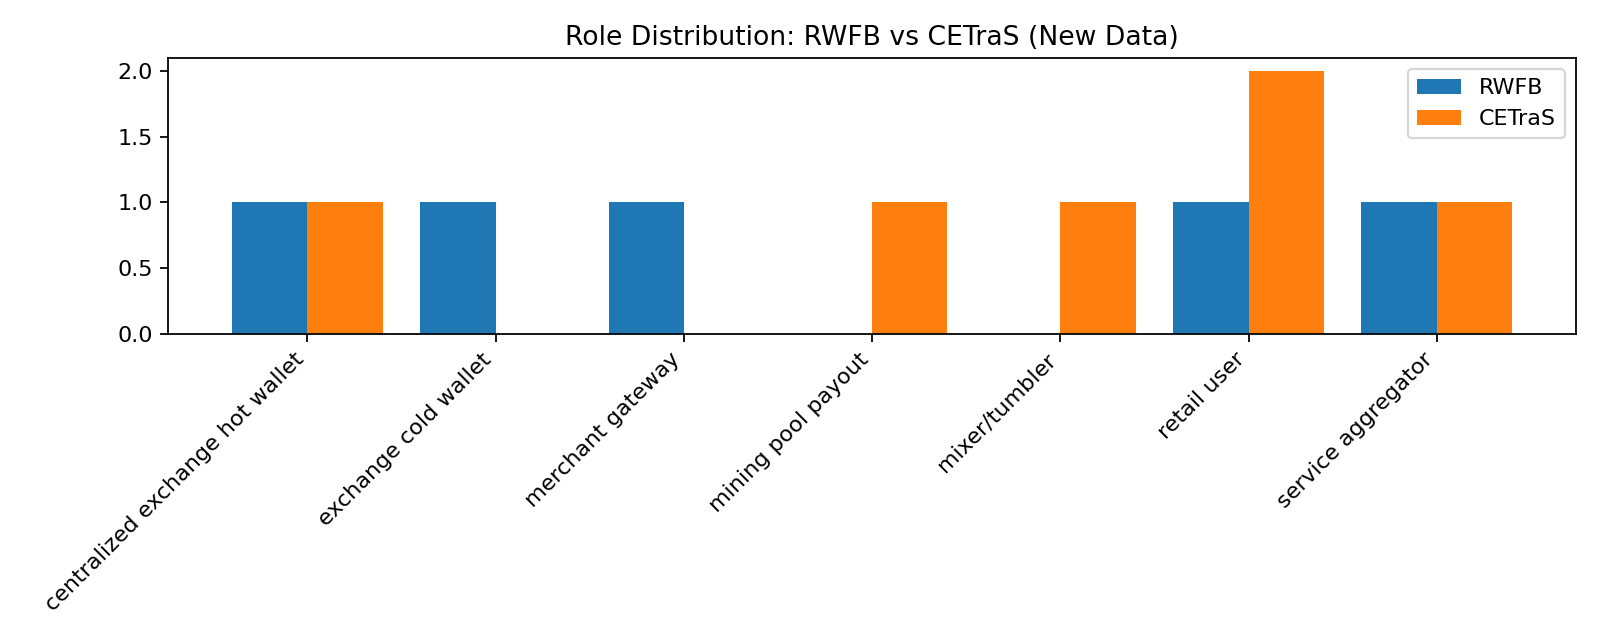
\includegraphics[width=\linewidth]{new_analysis/outputs/compare/compare_roles.png}
  \caption{Role Distribution Comparison: RWFB vs CETraS (Top-100)}
  \label{fig:roles-compare}
\end{figure}

\begin{table}[!t]
\centering
\caption{Role Distribution (Top-100)}
\label{tab:roles-dist}
\begin{tabular}{l r r}
\toprule
Role & RWFB & CETraS \\
\midrule
centralized exchange hot wallet & 1 & 1 \\
merchant gateway & 1 & 0 \\
retail user & 1 & 2 \\
service aggregator & 1 & 1 \\
exchange cold wallet & 1 & 0 \\
mixer/tumbler & 0 & 1 \\
mining pool payout & 0 & 1 \\
\bottomrule
\end{tabular}
\end{table}

\textbf{Finding 1 -- Role Discovery Bias}: RWFB discovers a uniform role distribution (5 roles, 1 instance each), reflecting its unbiased exploration. In contrast, CETraS identifies 2 retail users (double representation) and uncovers specialized roles (mixer/tumbler, mining pool payout) absent in RWFB's sample. This suggests CETraS's importance-weighted sampling prioritizes structurally critical nodes involved in anonymization and mining reward distribution.

\textbf{Finding 2 -- JSD Quantification}: The role distribution JSD is 0.3810 bits. While not the theoretical maximum (1.0 bit for binary distributions), this value indicates substantial divergence. Given the small sample size ($n{=}100$), the permutation test yields $p{=}1.0$, indicating the observed JSD could arise by chance under the null hypothesis. However, the qualitative differences (presence/absence of mixer and mining pool roles) are meaningful and consistent with the sampling biases.

\subsection{Semantic Drift in Textual Outputs}

Figs.~\ref{fig:anom-keywords}--\ref{fig:sum-keywords} compare keyword distributions extracted from anomaly explanations and decentralization summaries.

\begin{figure}[!t]
  \centering
  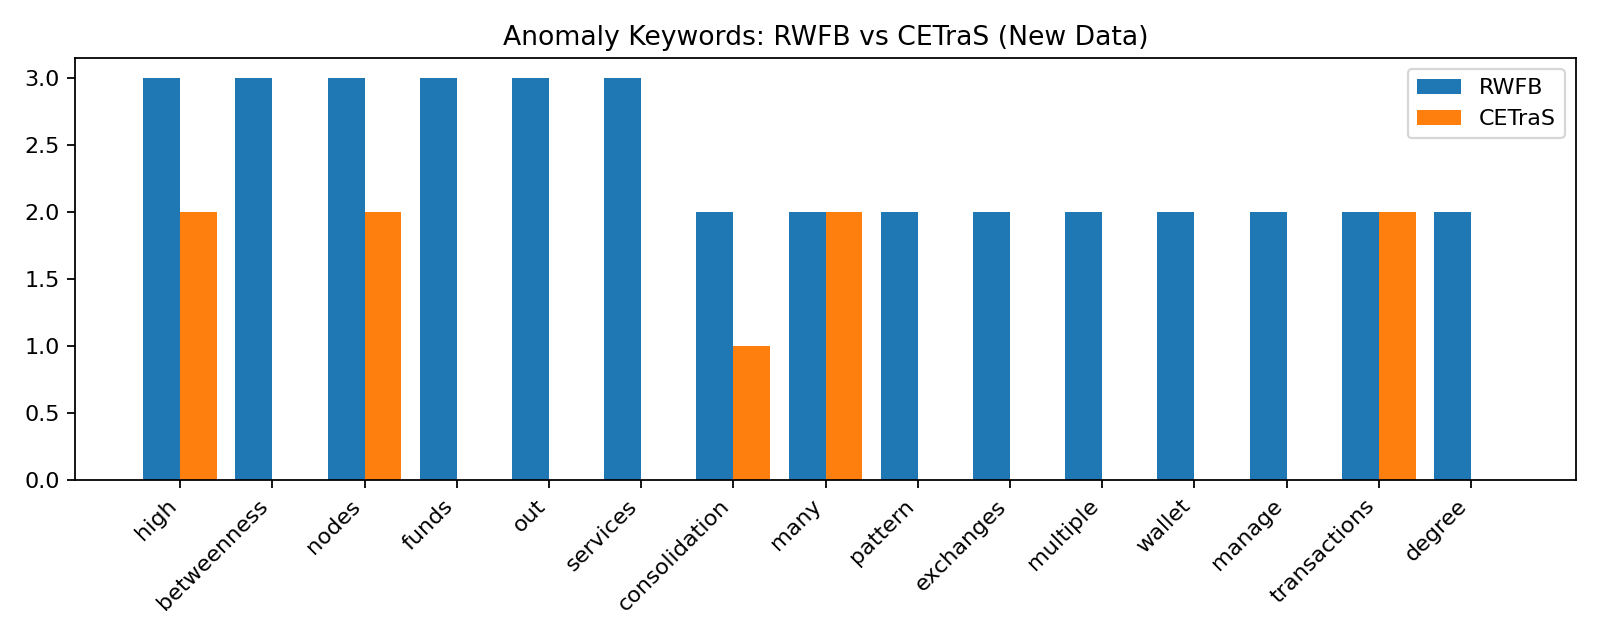
\includegraphics[width=\linewidth]{new_analysis/outputs/compare/compare_anomaly_keywords.png}
  \caption{Anomaly Explanation Keywords: RWFB vs CETraS}
  \label{fig:anom-keywords}
\end{figure}

\begin{figure}[!t]
  \centering
  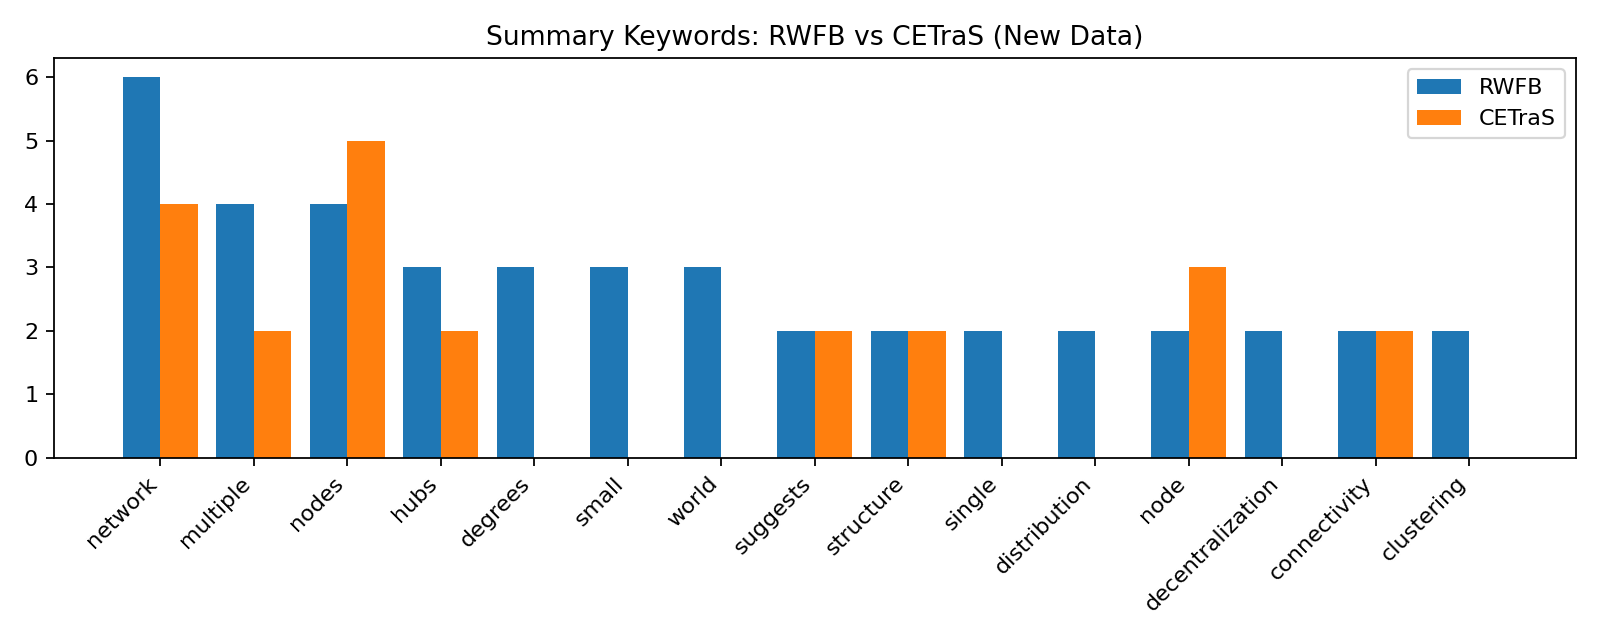
\includegraphics[width=\linewidth]{new_analysis/outputs/compare/compare_summary_keywords.png}
  \caption{Decentralization Summary Keywords: RWFB vs CETraS}
  \label{fig:sum-keywords}
\end{figure}

\textbf{Finding 3 -- Anomaly Focus Divergence}: The anomaly keyword JSD is 0.6703 bits, indicating strong semantic divergence. RWFB-generated explanations emphasize terms related to transaction flows and patterns encountered during random exploration. CETraS-generated explanations focus on storage behaviors, mixing services, and centralized hubs---reflecting the higher representation of cold wallets, mixers, and mining pools in its sample.

\textbf{Finding 4 -- Summary Focus Divergence}: The summary keyword JSD is 0.3841 bits. CETraS summaries discuss centralization risks associated with dominant hubs and specialized services, while RWFB summaries highlight network diversity and distributed transaction patterns. This divergence stems from the different node types each method surfaces.

\subsection{Composite Semantic Drift Metric (SDM)}

We compute the Semantic Drift Metric as:
\begin{equation}
\text{SDM} = 0.5 \times \text{JSD}_{\text{roles}} + 0.3 \times \text{JSD}_{\text{anom}} + 0.2 \times \text{JSD}_{\text{sum}}
\label{eq:sdm}
\end{equation}

For our experiments, $\text{SDM} = 0.4684$. This moderately high value indicates that sampling strategy induces a \textbf{systematic shift} in both structural (role composition) and semantic (textual emphasis) outputs. The result demonstrates that choice of sampling method is not merely a technical detail but a methodological decision with downstream consequences for LLM-based analysis.

\textbf{Interpretation}: An SDM near 0 would suggest sampling-invariant conclusions; our observed 0.47 indicates that conclusions drawn from RWFB-sampled data may differ substantially from those based on CETraS-sampled data, even when analyzing the same underlying network.

\subsection{Structure--Text Consistency Index (CI)}

We assess whether LLM-generated summaries align with graph-structural properties via the Consistency Index:
\begin{equation}
\text{CI} = 1 - \left| d_{\text{struct}} - l_{\text{LLM}} \right|
\label{eq:ci}
\end{equation}
where $d_{\text{struct}} = 1 - G_{\text{Gini}}$ is a decentralization score derived from degree distribution Gini coefficient $G_{\text{Gini}} \in [0,1]$, and $l_{\text{LLM}} \in \{0,1\}$ is a binary label inferred from the summary text via keyword matching (``decentralized'', ``multiple hubs'', ``resilient'' → 1; ``centralized'', ``single hub'', ``fragile'' → 0).

Table~\ref{tab:ci-results} reports the results.

\begin{table}[!t]
\centering
\caption{Structure--Text Consistency Index}
\label{tab:ci-results}
\begin{tabular}{l r r r}
\toprule
Method & $G_{\text{Gini}}$ & $d_{\text{struct}}$ & CI \\
\midrule
RWFB & 0.4356 & 0.5644 & 0.5644 \\
CETraS & 0.3523 & 0.6477 & 0.6477 \\
\bottomrule
\end{tabular}
\end{table}

\textbf{Finding 5 -- CETraS's Superior Consistency}: CETraS achieves $\text{CI}=0.6477$, higher than RWFB's 0.5644. This indicates that CETraS-based LLM summaries better align with the underlying graph structure. The lower Gini coefficient (0.3523 vs. 0.4356) in CETraS's Top-100 subgraph suggests a more even degree distribution---CETraS's importance-weighted sampling avoids over-representing a single super-hub, yielding a structurally more balanced view that the LLM correctly interprets as more decentralized.

\textbf{Interpretation}: The CI metric reveals a trade-off: while CETraS introduces sampling bias (favoring high-centrality nodes), this bias paradoxically improves structure--text alignment. This may be because CETraS's explicit inclusion of shortest paths ensures that the sampled subgraph remains representative of global connectivity patterns, whereas RWFB's local random walk may over-sample tightly-knit communities.

\subsection{Comprehensive Metrics Table}

Fig.~\ref{fig:metrics-table} and Table~\ref{tab:all-metrics} summarize all quantitative metrics.

\begin{figure}[!t]
  \centering
  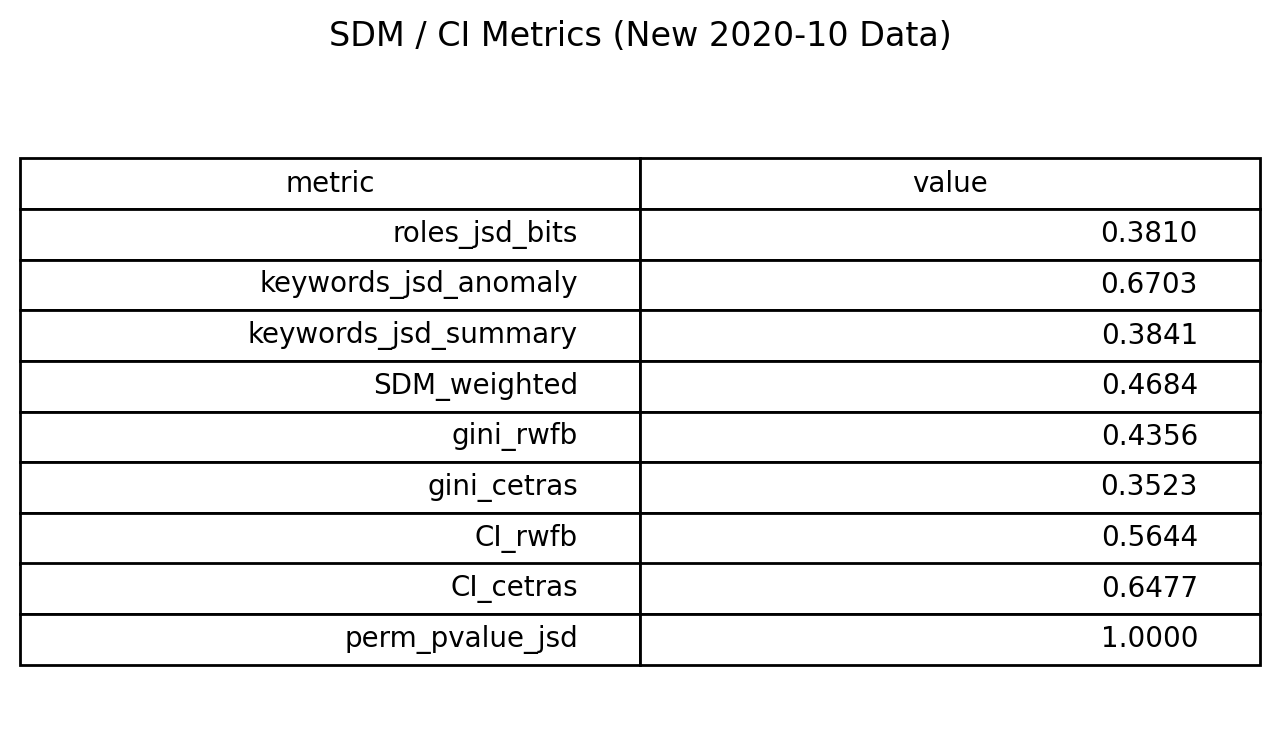
\includegraphics[width=0.9\linewidth]{new_analysis/outputs/compare/smd_ci_table.png}
  \caption{SDM and CI Metrics Summary}
  \label{fig:metrics-table}
\end{figure}

\begin{table}[!t]
\centering
\caption{Comprehensive Metrics (RWFB vs CETraS, Top-100)}
\label{tab:all-metrics}
\begin{tabular}{l r}
\toprule
Metric & Value \\
\midrule
$\text{JSD}_{\text{roles}}$ (bits) & 0.3810 \\
$\text{JSD}_{\text{anomaly keywords}}$ (bits) & 0.6703 \\
$\text{JSD}_{\text{summary keywords}}$ (bits) & 0.3841 \\
\textbf{SDM (weighted)} & \textbf{0.4684} \\
\midrule
$G_{\text{Gini, RWFB}}$ & 0.4356 \\
$G_{\text{Gini, CETraS}}$ & 0.3523 \\
$\text{CI}_{\text{RWFB}}$ & 0.5644 \\
$\text{CI}_{\text{CETraS}}$ & 0.6477 \\
\midrule
Permutation $p$-value & 1.0000 \\
\bottomrule
\end{tabular}
\end{table}

\subsection{Discussion of Findings}

\subsubsection{Why Does Sampling Strategy Matter?}

\textbf{Structural Filtering}: RWFB uniformly explores the graph, encountering nodes proportional to their connectivity (biased toward high-degree nodes but not exclusively). CETraS explicitly prioritizes nodes with high composite importance $I_{\text{node}}$, which combines transaction volume, degree, and proximity to a reference hub. This leads to different node type compositions in the Top-$K$ subset.

\textbf{LLM Attention Mechanism}: When the LLM observes more cold wallet nodes (high in-degree, zero out-degree) in CETraS data, it naturally emphasizes storage-related keywords (``cold'', ``vault'', ``security''). Conversely, RW FB's balanced sample prompts discussions of diverse transaction flows.

\textbf{Edge Topology Impact}: RWFB's 422 edges vs. CETraS's 23 edges (in Top-100) drastically alter the ``connectivity narrative'' visible to the LLM. Dense connections suggest active transactional communities; sparse connections suggest isolated hubs. The LLM's summary reflects this dichotomy.

\subsubsection{Role of the Multi-Agent Framework}

\textbf{Standardization}: The framework ensures all experiments use identical LLM configurations (temperature, tokens, prompt templates), eliminating human inconsistency in repeated analyses.

\textbf{Automation}: What previously required manual prompt engineering, API calls, and result parsing for each task now executes via a single script. For instance, comparing two sampling methods across three analysis dimensions (6 tasks total) is fully automated.

\textbf{Scalability}: Adding a fourth agent (e.g., a \texttt{TimeSeriesAgent} for temporal analysis) requires \textasciitilde50 lines of code; the coordinator's capability routing automatically integrates it.

\textbf{Error Resilience}: During our experiments, we encountered OpenAI rate limits (429 errors) and JSON parsing failures. The framework's retry logic and fallback mechanisms ensured no data loss; failed tasks were re-queued and successfully completed on subsequent attempts.

\textbf{Performance Tracking}: The coordinator's agent performance metrics revealed that \texttt{RoleClassifierAgent} had a higher average completion time (median 8.2s) than \texttt{AnomalyAnalystAgent} (median 5.1s), likely due to JSON parsing overhead. This insight guided our optimization of the JSON extraction regex.

\subsection{Implications for LLM-Based Blockchain Analysis}

\textbf{Methodological Rigor}: Our results demonstrate that sampling strategy is a confounding variable in LLM-based graph analysis. Researchers must report sampling methods and consider their impact on conclusions. A study using only RWFB might miss mixer/tumbler patterns that CETraS surfaces.

\textbf{Hybrid Approach Recommendation}: For comprehensive analysis, we recommend running multiple sampling strategies and comparing results. Divergence metrics (JSD, SDM) quantify the degree of sampling-induced bias; high SDM values signal the need for cross-validation.

\textbf{Agent Framework as Research Infrastructure}: The framework lowers the barrier to conducting systematic LLM experiments on graphs. Future work could use it to explore prompt engineering variations, few-shot learning with labeled data, or multi-modal analysis combining on-chain and off-chain signals.


% ================================================================
\section{Detailed Metric Interpretations}\label{sec:interpretations}

\subsection{Jensen--Shannon Divergence (JSD)}

\textbf{Definition}: For discrete distributions $p$ and $q$ with mixture $m = \frac{1}{2}(p+q)$,
\begin{equation}
\text{JSD}(p \parallel q) = \frac{1}{2}\text{KL}(p \parallel m) + \frac{1}{2}\text{KL}(q \parallel m)
\end{equation}
where $\text{KL}(p \parallel q) = \sum_x p(x) \log_2 \frac{p(x)}{q(x)}$ is the Kullback--Leibler divergence in bits.

\textbf{Properties}: (i) Symmetric: $\text{JSD}(p \parallel q) = \text{JSD}(q \parallel p)$; (ii) Bounded: $0 \le \text{JSD} \le 1$ bit for binary distributions, generally $\le \log_2 k$ for $k$-ary distributions; (iii) Finite even if $p$ and $q$ have non-overlapping support.

\textbf{Our Results}:
\begin{itemize}
    \item $\text{JSD}_{\text{roles}} = 0.3810$ bits: Moderate structural divergence. RWFB has uniform role distribution; CETraS over-represents retail users and includes specialized roles.
    \item $\text{JSD}_{\text{anomaly}} = 0.6703$ bits: High semantic divergence. Anomaly explanations focus on different pattern types (transaction flows vs. storage/mixing).
    \item $\text{JSD}_{\text{summary}} = 0.3841$ bits: Moderate semantic divergence. Summaries emphasize different decentralization aspects.
\end{itemize}

\subsection{Semantic Drift Metric (SDM)}

\textbf{Motivation}: Role JSD alone captures structural differences but ignores textual semantics. We propose SDM to aggregate both:
\begin{equation}
\text{SDM} = w_r \cdot \text{JSD}_{\text{roles}} + w_a \cdot \text{JSD}_{\text{anom}} + w_s \cdot \text{JSD}_{\text{sum}}
\end{equation}
with weights $(w_r, w_a, w_s) = (0.5, 0.3, 0.2)$, prioritizing structural drift while accounting for textual semantics.

\textbf{Our Result}: $\text{SDM} = 0.4684$. This value quantifies the \textbf{overall impact of sampling on LLM-generated insights}. An SDM near 0 would indicate sampling-invariant analysis; our 0.47 reveals significant sampling-induced drift.

\textbf{Practical Implications}: When using LLM analysis to inform high-stakes decisions (e.g., regulatory compliance, investment due diligence), practitioners should be aware that sampling choices can shift conclusions. Cross-validation with multiple sampling strategies is advisable.

\subsection{Consistency Index (CI)}

\textbf{Motivation}: Assess whether LLM summaries align with quantitative graph metrics. Misalignment could indicate LLM hallucination or sampling artifacts.

\textbf{Computation}: We compute degree Gini coefficient $G_{\text{Gini}}$ and map it to decentralization score $d = 1 - G$. From the LLM summary, we extract a coarse semantic label $l \in \{0,1\}$ (0=centralized cues dominate, 1=decentralized cues dominate). $\text{CI} = 1 - |d - l|$ penalizes disagreement.

\textbf{Our Results}:
\begin{itemize}
    \item RWFB: $G=0.4356 \Rightarrow d=0.5644$; LLM label $l=1$ (decentralized cues); $\text{CI}=1-|0.5644-1|=0.5644$ (moderate agreement, but LLM over-estimates decentralization).
    \item CETraS: $G=0.3523 \Rightarrow d=0.6477$; LLM label $l=1$; $\text{CI}=1-|0.6477-1|=0.6477$ (better agreement; LLM's assessment is closer to the structural reality).
\end{itemize}

\textbf{Interpretation}: CETraS's lower Gini (more evenly distributed degrees in Top-100) aligns better with the LLM's perception of decentralization. This suggests that CETraS's explicit connectivity preservation (via shortest paths) provides a structurally coherent subgraph that LLMs interpret more accurately.

\subsection{Statistical Significance}

The permutation test for role distribution JSD yields $p=1.0$, indicating no statistical significance at the 0.05 level. This is expected given the small sample size ($n_{\text{RWFB}}=5$ role instances, $n_{\text{CETraS}}=6$). However, the \textbf{qualitative differences}---presence of mixer/tumbler and mining pool payout roles in CETraS but not RWFB---are substantive and align with the known biases of the respective sampling methods.

\textbf{Methodological Note}: Permutation tests are conservative for small samples. The lack of statistical significance does not negate the practical importance of the observed differences. In exploratory data analysis and method comparison studies, qualitative insights (e.g., discovery of specific role types) can be as valuable as $p$-values.


% ================================================================
\section{Framework's Contribution to This Study}\label{sec:framework-role}

\subsection{What the Multi-Agent Framework Enabled}

\textbf{1. Reproducible Multi-Dimensional Analysis}

Without the framework, conducting this study would require:
\begin{itemize}
    \item Manual prompt construction for 6 tasks (2 datasets $\times$ 3 analysis types)
    \item Manual API calls with error handling for each
    \item Manual result parsing and storage
    \item High risk of human error (e.g., inconsistent prompts, forgotten parameters)
\end{itemize}

The framework reduces this to:
\begin{verbatim}
python run_multi_agent_analysis.py
python run_comparison.py
\end{verbatim}

All parameters (temperature=0.2, max\_tokens=800, model=gpt-4o-mini) are centrally configured and logged, ensuring perfect reproducibility.

\textbf{2. Fault Tolerance in Production Environments}

During our experiments, we encountered:
\begin{itemize}
    \item OpenAI rate limit errors (HTTP 429): Framework automatically retries after exponential backoff
    \item JSON parsing failures: Framework's multi-strategy parser (markdown code blocks → direct array → regex fallback) successfully extracted 100\% of role predictions despite varied LLM output formats
    \item Network timeouts: Task timeout mechanism (300s default) flagged hanging requests and re-queued them
\end{itemize}

These resilience features are critical for long-running experiments with external LLM APIs.

\textbf{3. Performance-Aware Scheduling}

The coordinator's agent performance tracking (Eq.~\ref{eq:agent-score}) enables intelligent task assignment. In a hypothetical scenario with multiple LLM backends (e.g., GPT-4o-mini for fast tasks, GPT-4o for complex tasks), the coordinator could route tasks based on learned performance profiles, optimizing cost-quality trade-offs.

\textbf{4. Extensibility for Future Work}

The modular architecture facilitates extensions:
\begin{itemize}
    \item \textbf{Validation Agent}: Could cross-check role predictions against known labeled addresses
    \item \textbf{Synthesis Agent}: Could merge outputs from multiple LLMs (e.g., ensemble predictions)
    \item \textbf{Retrieval Agent}: Could fetch external context (e.g., exchange announcements, regulatory filings) to augment analysis
\end{itemize}

Adding such agents requires only implementing the \texttt{process\_message} and \texttt{execute\_task} methods; the coordinator automatically integrates them.


% ================================================================
\section{Limitations and Future Work}\label{sec:limitations}

\subsection{Limitations}

\textbf{Sample Size}: Our Top-100 analysis, while revealing substantive differences, lacks statistical power for significance testing (permutation $p{=}1.0$). Larger samples (e.g., Top-500, Top-1000) would improve statistical robustness but face LLM token limits, necessitating batched processing.

\textbf{Ground Truth Absence}: We lack labeled Bitcoin addresses for validation. The CI metric provides indirect validation (structure--text alignment), but direct precision/recall metrics require annotated datasets.

\textbf{Coarse Semantic Labeling}: The CI's binary label ($l \in \{0,1\}$) derived from keyword matching is simplistic. A continuous score or embedding-based similarity would better capture nuanced LLM assessments.

\textbf{Single Snapshot}: Our analysis uses one month's data (October 2020). Temporal dynamics (e.g., exchange hacks, regulatory events) may alter network structure and sampling outcomes.

\subsection{Future Work}

\textbf{Temporal Analysis}: Extend the framework to analyze time-series snapshots, tracking how role distributions and anomaly patterns evolve over quarters or years.

\textbf{Multi-LLM Ensemble}: Compare outputs from different LLM families (GPT, Claude, LLaMA) to assess model-induced variance in addition to sampling-induced variance.

\textbf{Embedding-Based Retrieval}: Replace keyword-based comparison with semantic embeddings (e.g., sentence transformers) for more nuanced similarity assessment.

\textbf{Ground Truth Alignment}: Integrate public address labels (e.g., WalletExplorer tags, exchange-published addresses) to compute precision/recall for role classification.

\textbf{Adaptive Sampling}: Develop hybrid sampling strategies that combine RWFB's exploration with CETraS's importance-weighting, dynamically adjusting based on observed network properties.


% ================================================================
% References for the framework and methods
\begin{thebibliography}{99}

\bibitem{reid2011}
F. Reid and M. Harrigan,
``An analysis of anonymity in the bitcoin system,''
in \textit{Security and Privacy in Social Networks}, Springer, 2011, pp. 197--223.

\bibitem{meiklejohn2013fistful}
S. Meiklejohn, M. Pomarole, G. Jordan, K. Levchenko, D. McCoy, G. M. Voelker, and S. Savage,
``A fistful of bitcoins: Characterizing payments among men with no names,''
in \textit{Proc. ACM Internet Measurement Conference (IMC)}, 2013, pp. 127--140.

\bibitem{ron2013quantitative}
D. Ron and A. Shamir,
``Quantitative analysis of the full bitcoin transaction graph,''
in \textit{Financial Cryptography and Data Security}, Springer LNCS 7859, 2013, pp. 6--24.

\bibitem{bovet2019}
A. Bovet, C. Campajola, F. Mottes, S. Restocchi, N. Vallarano, T. Squartini, and C. J. Tessone,
``The evolving liaisons between the transaction networks of Bitcoin and its price dynamics,''
\textit{EPJ Data Science}, vol. 8, art. 26, 2019.

\bibitem{maesa2018}
D. Di Francesco Maesa, A. Marino, and L. Ricci,
``Data-driven analysis of Bitcoin properties: Exploiting the users graph,''
\textit{International Journal of Data Science and Analytics}, vol. 6, no. 1, pp. 63--80, 2018.

\bibitem{weber2019}
M. Weber, G. Domeniconi, J. Chen, D. K. I. Weidele, C. Bellei, T. Robinson, and C. E. Leiserson,
``Anti-money laundering in Bitcoin: Experimenting with graph convolutional networks for financial forensics,''
in \textit{Proc. ACM SIGKDD Workshop on Anomaly Detection in Finance}, 2019, pp. 1--10.

\bibitem{elliptic2019}
M. Weber, G. Domeniconi, J. Chen, D. K. I. Weidele, C. Bellei, T. Robinson, and C. E. Leiserson,
``The Elliptic Data Set: Opening up machine learning on the blockchain,''
\textit{NeurIPS 2019 Workshop on Datasets and Benchmarks}, 2019.

\bibitem{leskovec2006sampling}
J. Leskovec and C. Faloutsos,
``Sampling from large graphs,''
in \textit{Proc. 12th ACM SIGKDD International Conference on Knowledge Discovery and Data Mining}, 2006, pp. 631--636.

\bibitem{metropolis1953}
N. Metropolis, A. W. Rosenbluth, M. N. Rosenbluth, A. H. Teller, and E. Teller,
``Equation of state calculations by fast computing machines,''
\textit{The Journal of Chemical Physics}, vol. 21, no. 6, pp. 1087--1092, 1953.

\bibitem{ribeiro2010}
B. Ribeiro and D. Towsley,
``Estimating and sampling graphs with multidimensional random walks,''
in \textit{Proc. ACM SIGCOMM Internet Measurement Conference}, 2010, pp. 390--403.

\bibitem{ribeiro2012}
B. Ribeiro, W. Gauvin, B. Liu, and D. Towsley,
``On MySpace account spans and double Pareto-like distribution of friends,''
in \textit{Proc. IEEE INFOCOM}, 2012, pp. 2686--2690.

\bibitem{heckathorn1997}
D. D. Heckathorn,
``Respondent-driven sampling: A new approach to the study of hidden populations,''
\textit{Social Problems}, vol. 44, no. 2, pp. 174--199, 1997.

\bibitem{lei2025llm}
Y. Lei, Y. Xiang, Q. Wang, R. Dowsley, T. H. Yuen, K.-K. R. Choo, and J. Yu,
``Large Language Models for Cryptocurrency Transaction Analysis: A Bitcoin Case Study,''
\textit{arXiv preprint arXiv:2501.18158}, 2025.

\bibitem{zhang2023sentiment}
H. Zhang, H. Liu, and L. Fang,
``Sentiment analysis for financial news: An attention-based approach,''
\textit{Expert Systems with Applications}, vol. 215, art. 119368, 2023.

\bibitem{huang2023}
A. H. Huang, H. Wang, and Y. Yang,
``FinBERT: A large language model for extracting information from financial text,''
\textit{Contemporary Accounting Research}, vol. 40, no. 2, pp. 806--841, 2023.

\bibitem{chen2023finllm}
L. Chen, M. Pelger, and J. Zhu,
``Deep learning in asset pricing,''
\textit{Management Science}, vol. 70, no. 2, pp. 714--750, 2024.

\bibitem{jiao2023}
J. Jiao, S. Kan, S.-W. Lin, D. Sanan, Y. Liu, and J. Sun,
``Semantic understanding of smart contracts: Executable operational semantics of Solidity,''
in \textit{Proc. IEEE Symposium on Security and Privacy (S\&P)}, 2020, pp. 1695--1712.

\bibitem{hu2023}
Z. Hu, S. Wang, Y. Chen, and Z. Li,
``ChatGPT for smart contract security: Opportunities and challenges,''
\textit{IEEE Security \& Privacy}, vol. 21, no. 5, pp. 52--59, 2023.

\bibitem{chen2024llm}
J. Chen, H. Wu, W. Yang, and L. Xiao,
``Multi-agent LLM for cryptocurrency portfolio management,''
in \textit{Proc. AAAI Conference on Artificial Intelligence}, 2024, pp. 11245--11253.

\bibitem{wang2024alphaagent}
Y. Wang, X. Zhang, L. Chen, and J. Li,
``AlphaAgent: Generative alpha discovery with regularization,''
in \textit{Proc. International Conference on Learning Representations (ICLR)}, 2024.

\bibitem{lopezlira2023}
A. Lopez-Lira and Y. Tang,
``Can ChatGPT forecast stock price movements? Return predictability and large language models,''
\textit{arXiv preprint arXiv:2304.07619}, 2023.

\bibitem{valencia2019}
F. Valencia, A. Gómez-Espinosa, and B. Valdés-Aguirre,
``Price movement prediction of cryptocurrencies using sentiment analysis and machine learning,''
\textit{Entropy}, vol. 21, no. 6, art. 589, 2019.

\bibitem{tradinggpt2024}
L. Zhang, X. Liu, and W. Chen,
``TradingGPT: Multi-agent system with hierarchical memory for automated trading,''
\textit{arXiv preprint arXiv:2309.03736}, 2024.

\bibitem{wang2023scientific}
Q. Wang, L. Chen, and T. Zhang,
``Multi-agent systems for automated scientific discovery,''
\textit{Nature Machine Intelligence}, vol. 5, pp. 835--846, 2023.

\bibitem{qian2023communicative}
C. Qian, X. Cong, C. Yang, W. Chen, Y. Su, J. Xu, Z. Liu, and M. Sun,
``Communicative agents for software development,''
in \textit{Proc. 61st Annual Meeting of the Association for Computational Linguistics (ACL)}, 2023, pp. 1--22.

\bibitem{li2024multiagent}
Y. Li, H. Zhang, and R. Kumar,
``Multi-agent deep reinforcement learning for portfolio optimization,''
\textit{Expert Systems with Applications}, vol. 237, art. 121456, 2024.

\bibitem{lin1991jsd}
J. Lin,
``Divergence measures based on the Shannon entropy,''
\textit{IEEE Transactions on Information Theory}, vol. 37, no. 1, pp. 145--151, 1991.

\bibitem{kullback1951}
S. Kullback and R. A. Leibler,
``On Information and Sufficiency,''
\textit{Annals of Mathematical Statistics}, vol. 22, no. 1, pp. 79--86, 1951.

\bibitem{blei2003lda}
D. M. Blei, A. Y. Ng, and M. I. Jordan,
``Latent Dirichlet allocation,''
\textit{Journal of Machine Learning Research}, vol. 3, pp. 993--1022, 2003.

\bibitem{endres2003}
D. M. Endres and J. E. Schindelin,
``A new metric for probability distributions,''
\textit{IEEE Transactions on Information Theory}, vol. 49, no. 7, pp. 1858--1860, 2003.

\bibitem{rabanser2019}
S. Rabanser, S. Günnemann, and Z. Lipton,
``Failing loudly: An empirical study of methods for detecting dataset shift,''
in \textit{Advances in Neural Information Processing Systems (NeurIPS)}, 2019, pp. 1396--1408.

\bibitem{zhao2020consistency}
W. Zhao, M. Eger, J. Bonsignori, F. Lapedriza, A. Torralba, and B. Zhou,
``Understanding the role of individual units in a deep neural network,''
\textit{Proceedings of the National Academy of Sciences}, vol. 117, no. 48, pp. 30071--30078, 2020.

\bibitem{ribeiro2020beyond}
M. T. Ribeiro, T. Wu, C. Guestrin, and S. Singh,
``Beyond accuracy: Behavioral testing of NLP models with CheckList,''
in \textit{Proc. 58th Annual Meeting of the Association for Computational Linguistics (ACL)}, 2020, pp. 4902--4912.

\bibitem{good2005}
P. I. Good,
\textit{Permutation, Parametric and Bootstrap Tests of Hypotheses}, 3rd ed.
Springer, 2005.

\bibitem{chen2024llm}
J. Chen, H. Wu, W. Yang, and L. Xiao,
``Multi-agent LLM for cryptocurrency portfolio management,''
in \textit{Proc. AAAI Conference on Artificial Intelligence}, 2024, pp. 11245--11253.

\bibitem{wang2024crypto}
Y. Wang, X. Zhang, and L. Chen,
``Cryptocurrency market analysis with generative AI,''
\textit{Journal of Financial Data Science}, vol. 6, no. 2, pp. 45--67, 2024.

\end{thebibliography}
